\newpage
\section{Firmware engineering}
\label{sec:fw}


\subsection{Firmware architecture}

\begin{figure}[ht]
    \centering
    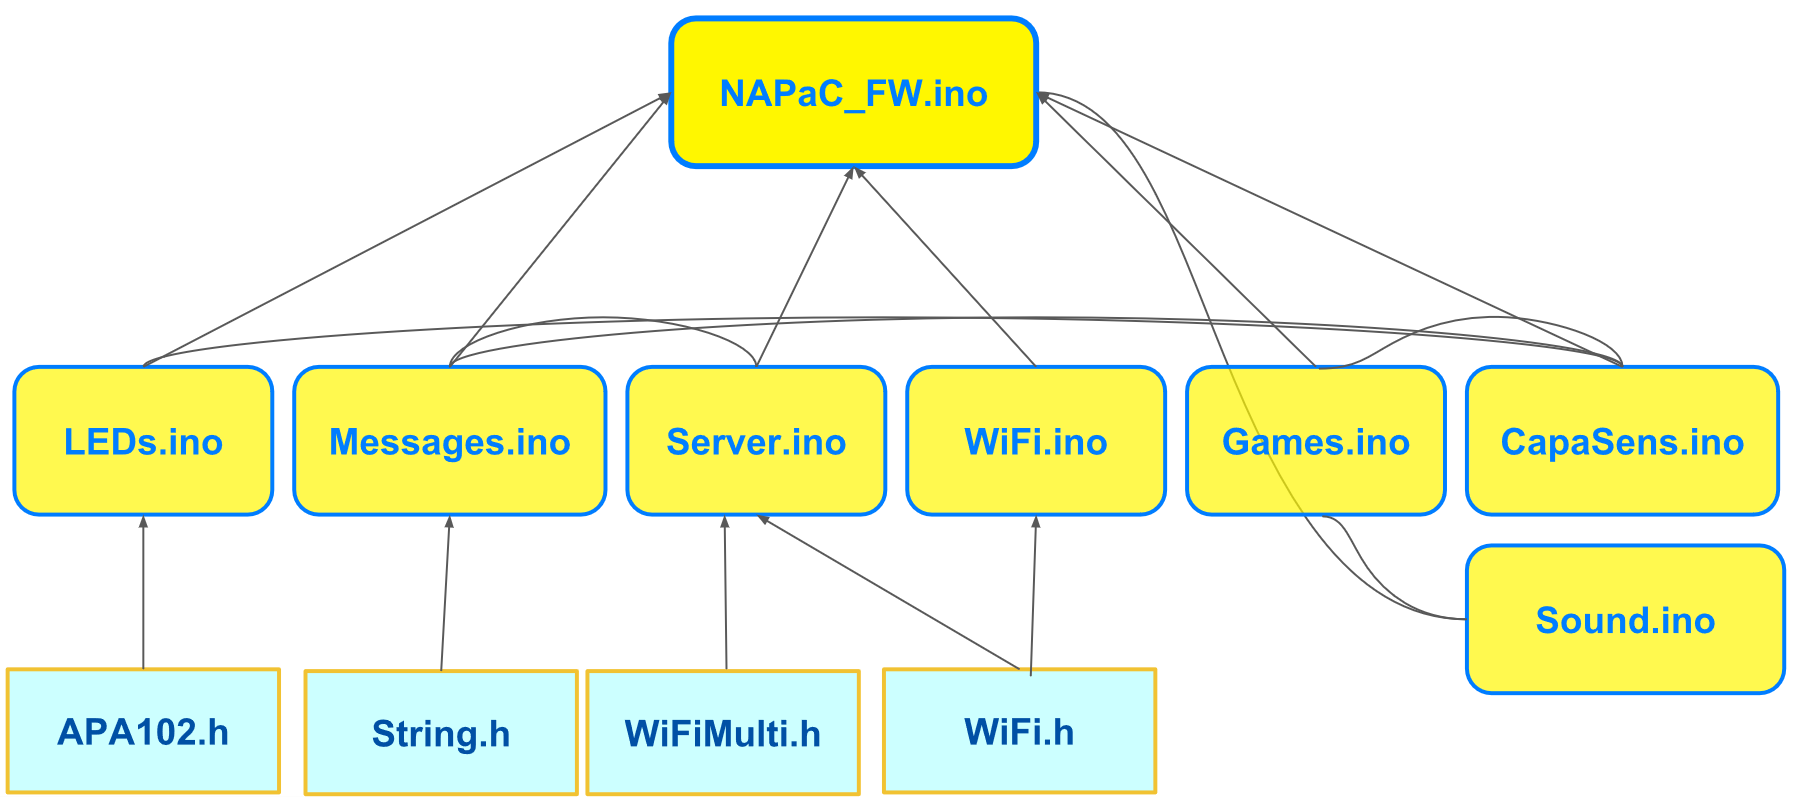
\includegraphics[width=0.8\textwidth]{images/FW/FW_architecture.PNG}
    \caption{Firmware architecture diagram with units and libraries}
    \label{fig:FW_architecture}
\end{figure}

The chosen architecture for our Arduino program is illustrated in Figure \ref{fig:FW_architecture}. The main file (NAPaC\_FW.ino) calls each separate unit which may call eachother depending on the implemented functions.
Each unit described below is conceived as a "library", with each its setup function(s) and functions relative to a hardware component or interaction.

\begin{description}[align=left]
\item  [NAPaC\_FW.ino] Used as the main file for our firmware. Runs through setup functions for each unit then calls the other functions (game interaction) from the loop. 
\item [LEDs.ino] Based on the APA102 library, this unit defines LED pins and sets up LED strips and output pins during setup. In this unit, we define main actions for LEDs such as turning on in a given colour, blinking, and turning on the LEDs in appropriate colours according to the game steps defined in figure \ref{fig:game_diagram}.
\item[Messages.ino] This unit defines the "alphabet" in accordance with the communication protocol defined in Table \ref{tab:comm_message}. This unit also holds functions for sending defined interaction messages to the server.
\item[Server.ino] The Server module has functions for connecting to the server, reading and sending messages as well as to close server connection. 
\item[Games.ino] The Games unit is the main file for interactions. It has functions defining a solo game and the game with parents, and keeps record of the Zone status (off, on, colour) for the plush toy. It also has functions defining the beginning and end of game sessions which interact with the server to begin and end game sessions.
\item[CapaSens.ino] In this unit, we set up the capacitive touch sensors and define the touch status with the touch library provided by ESP32. 
\item[Sound.ino] The Sound unit enables the microcontroller to play sounds through the buzzer. We have defined the standard Western musical scale (Do-Re-Mi-...) and implemented several sound tests and jingles for the games. 
\end{description}



    \paragraph{Choice of coding environment}
After experimenting with both ESP32 Eclipse framework and the Arduino environment, we decided to chose Arduino as our coding platform for the widely available examples and ease of programming.
    \paragraph{Libraries}
In our project, we use libraries for the APA102 LEDs from Polulu \cite{apa102-arduino}, as well as WiFi configuration and capacitive touch sensors libraries from Espressif \cite{esp32-arduino}. Their main parameters and working principles are described below. 

\subsection{Firmware Flow chart}

The diagram below illustrates the behaviour of the plush toy's firmware. The detailed flow chart for the game session can be found in figure \ref{fig:game_diagram}.

\begin{figure}[ht]
    \centering
    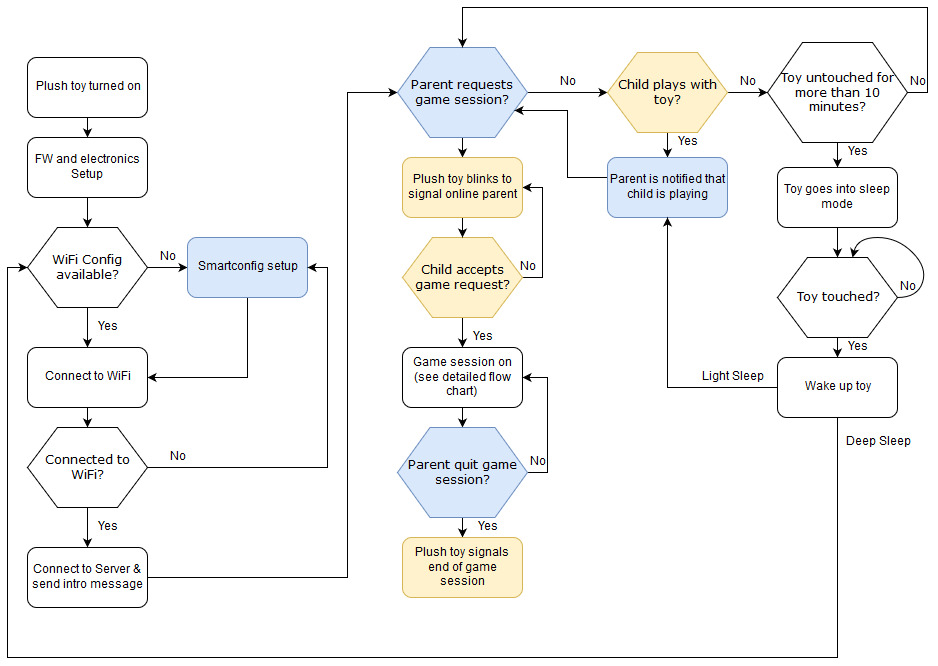
\includegraphics[width=0.9\textwidth]{images/FW/FW_diagram.jpg}
    \caption{Firmware Flow chart}
    \label{fig:FW_flowchart}
\end{figure}
    
\newpage    
\subsection{Description of Functions}

\subsubsection{NAPaC\_FW}

\paragraph{Setup}
The setup function runs through the induvidual setup functions of each unit: LEDs, Capacitive Sensors, Sound. It then proceeds to find WiFi SmartConfig (or connect to WiFi using an existing one), connects to server then sends a "presentation" message to the server sending its ID.

\lstinputlisting[style=Arduino, firstline=13, lastline=26]{code_snippets/arduino/NAPaC_FW.ino}

\paragraph{Main Loop}
In the main loop, the program waits for a message requesting the beginning of a game session. In a final version of the firmware we could expect functions such as checking for child's presence, sleep mode, etc. 

\lstinputlisting[style=Arduino, firstline=28]{code_snippets/arduino/NAPaC_FW.ino}

\subsubsection{Messages}
The messages unit is used to define and send messages to the server. These messages are defined in Section \ref{subsec:communication}. 

\paragraph{Alphabet setup} This snippet of code sets up the characters required form the communication protocol. 
\lstinputlisting[style=Arduino, firstline=19, lastline=22]{code_snippets/arduino/Messages.ino}

\paragraph{first\_message} The microcontroller sends a message to the server with its unique identifier, allowing the server to link it with its IP address.
\lstinputlisting[style=Arduino]{code_snippets/arduino/first_message.txt}

\paragraph{accept\_game\_message} Sends the 2002 message meaning the child has accepted the parent's game request
\lstinputlisting[style=Arduino]{code_snippets/arduino/accept_game.txt}

\paragraph{LED\_on\_message} Sends message 2003 with LED ID of LED turned on by the child
\lstinputlisting[style=Arduino]{code_snippets/arduino/led_on.txt}

\paragraph{LED\_off\_message} Sends message 2004 with LED ID of LED turned off by the child. This message is very similar to message 2003 above. 
%\lstinputlisting[style=Arduino, firstline=60, lastline=67]{code_snippets/arduino/Messages.ino}

\paragraph{hello} Prints a welcoming message to serial.



\subsubsection{WiFi connectivity and Server communication}\label{subsec:fw/Functions/WiFi}
We use SmartConfig to send the WiFi configuration to the microcontroller from the parent's smartphone. The WiFi configuration can also be save to the program for easier programming. 
Our goal for China or next semester is to save a new SmartConfig to the EEPROM memory then retrieve it upon launch to connect to a known WiFi network. 
    
\paragraph{WiFi Smartconfig}
The ESP32 Arduino SmartConfig libraries allow us to easily connect to a WiFi with configuration send by a nearby smartphone. The SmartConfig protocol is described in detail in section \ref{subsubsec:android-smartconfig}. 
\medskip
We have also implemented a function to connected the microcontroller to a known WiFi network, which characteristics as for now hard-coded in the firmware. Our goal for next semester is to save a previously received configuration to the EEPROM, retrieve it, then connect to the WiFi network using this configuration, as well as save multiple configurations. 


%\lstinputlisting[style=Arduino, firstline=9, lastline=35]{code_snippets/arduino/WiFi.ino}

%The following function allows the microcontroller to connect to a hardcoded WiFi network.  
%\lstinputlisting[style=Arduino, firstline=37, lastline=53]{code_snippets/arduino/WiFi.ino}


\paragraph{Connection to server}
The code below allows the microcontroller to connect to the server in order to enable communications with the parent's smartphone. 
\lstinputlisting[style=Arduino]{code_snippets/arduino/server.txt}

\paragraph{Read message from server} This function reads a message sent by the parent's smartphone and transmitted through the server. It reads the message and saves it into a string that it returns. 
\lstinputlisting[style=Arduino]{code_snippets/arduino/read_message.txt}

\subsubsection{Games}
The main part of our firmware and most visible to the user is the "game" interaction. For now, we have set one type of interaction, or one game, but could imagine implementing other ones. A solo game is also available for testing. Figure \ref{fig:game_diagram} presents the flowchart for the game interaction. The goal of the "game" is that either the parent or child can chose to turn on one or several LEDs which will also light up on the game partner's device. A sound corresponding to the zone will also be played. The LEDs turn on the colour of the player who turned them on and the other player can turn them off and then on in their own colour. 

\begin{figure}[ht]
    \centering
    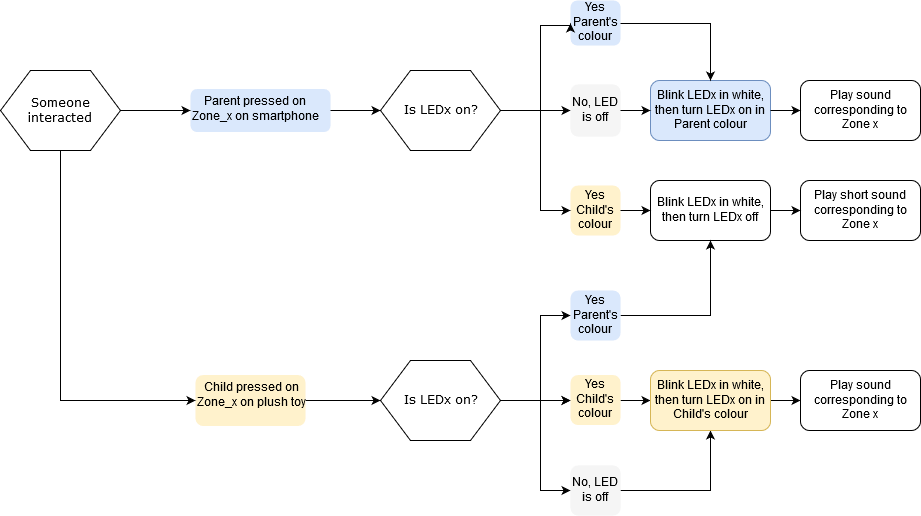
\includegraphics[width=\textwidth]{images/FW/FW_game_diagram.png}
    \caption{Flowchart for game interaction. Parent interactions are represented in blue while child interactions are in yellow.}
    \label{fig:game_diagram}
\end{figure}

\paragraph{Game functions}

\begin{description}[align=left]
\item[accept\_game\_request] Blinks the "heart" light and plays jingle to signal the parent wants to start a play session. When the child touches the plush toy the play session is immediately and automatically started and an accept message is sent to the server. 
\item[end\_game\_session] Is called when a parent requests the end of a game session. A jingle signalling the end of the game plays, and the heart LED blinks signalling the parent is going offline. All interaction LEDs turn off. 
\item[solo\_game] Is a test function allowing a solo game with the plush toy. The user can touch the sensors to turn successively on or off the LEDs in their own colour and play sound.
\item[parent\_game] Main game function, played between child and parent. This function waits for either a message from the server or for the child to touch the plush toy and turns on or off the LEDs accordingly, as described in figure \ref{fig:game_diagram}. 
\end{description}

\subsubsection{Capacitive touch sensors}\label{sec:capa_sens}

The capacitive touch sensors are crucial for the child's interaction with the plush toy. The functions used in the firmware are listed below. In the prototype presented in MS5, we only distinguished between touched and untouched, but hope to find the right settings to have a better sensitivity to different kinds of touching or pressing through the skin and plush stuffing. 

\paragraph{CapaSens Functions} 

\begin{description}[align=left]
\item[setup\_capa] Sets up the capacitive touch sensor pins as inputs then reads the initial value of each touch sensor.
\item[touch\_read\_value(touch\_id)] Reads the value on sensor of given ID. 
\item[capa\_touched(touch\_id)] Returns PRESSED if the touch sensor is being touched or RELEASED if not. Further improvement would include different states of touch (touch, light press or strong press).
\item[presence] Returns 1 if any sensor is touched, meaning the child is holding or playing with the plush toy.
\item[test\_touch\_values] Test function which prints the sensor values in serial.
\item[test\_if\_touched] Test function printing  the ID and value of any touched sensor in serial monitor.
\end{description}
    
\paragraph{Influence of sensing parameters}

\begin{figure}[ht]
    \centering
    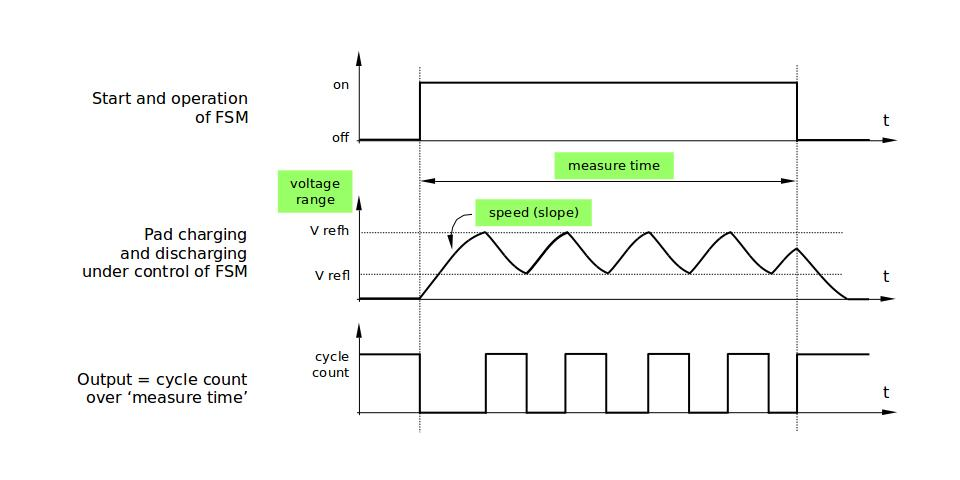
\includegraphics[width=0.8\textwidth]{images/FW/touch_parameters.jpg}
    \caption{ESP32 built-in touch sensor parameters}
    \label{fig:esp_touchparameters}
\end{figure}

The ESP32 built-in capacitive touch sensors have three parameters (illustrated in Fig. \ref{fig:esp_touchparameters}) that can be set by the user: measure time, voltage range and charge/discharge speed. These parameters will affect the sensitivity of the touch sensors. A slow charge/discharge cycle will lead to less sensitivity (illustrated with a test of different touches in figure \ref{fig:esp_touchtest}) while a fast cycle will lead to a high sensitivity. We still need to find the right set of parameters to ensure detection of touch through textile layer while limiting the risk of false positives and interference between sensors. With the right set of parameters, we will be able to detect and differentiate touch and press on a single touch sensor through layers of fabric. 




The Arduino environment does not allow easy tweaking of the capacitive touch sensors described in \ref{sec:capa_sens}. This can be done in C programs available from the ESP32 GitHub. We are still testing the parameters to find the right sensitivity and parameters, which depend on the shape and connections of the touch sensors.

\medskip The figure below (\ref{fig:esp_touchtest}) presents a touch test done with a steep measuring slope (as described in figure \ref{fig:esp_touchparameters}) and shows a high sensitivity to different types of touch such as touching, pressing or squeezing hard. However, in the Arduino environment, the default measurement speed is relatively slow, which strongly limits the sensitivity range of the sensors.

\begin{figure}[ht]
    \centering
    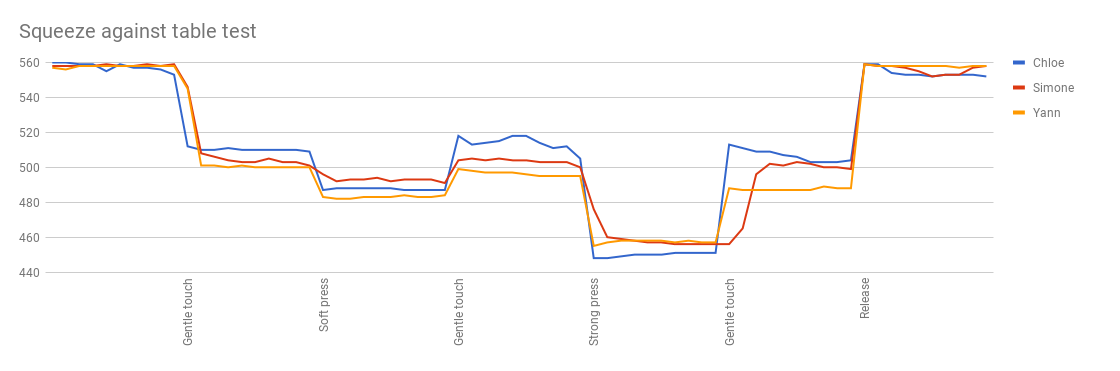
\includegraphics[width=\textwidth]{images/FW/capa_squeeze_table_multi.png}
    \caption{Test values for different touch/squeeze patterns with different users}
    \label{fig:esp_touchtest}
\end{figure}



\subsubsection{LEDs}\label{subsec:fw/Functions/LEDs}

The LEDs are connected as two LED strips on our microcontroller. We programmed several colours which can be used in the game and LED modes (on, off, blinking) to simplify other functions in the firmware. 

\paragraph{LED functions}

\begin{description}[align=left]
\item[setup\_LEDs] Sets up both LED strips and turns off LEDs
\item[all\_LED\_off] Switches off all LEDs
\item[set\_LED(LEDid, LED\_mode)] Turns on a LED in given colour, according to its positioning and LED strip.
\item[blink\_LED(LEDid, LED\_mode)] Blinks a LED over 1 second. 
\item[game\_set\_LED(LEDid, LED\_mode)] Function called from parent\_game which turns on or off LEDs and updates zone status according to its previous status and interaction. 
\end{description}

\lstinputlisting[style=Arduino, firstline=98, lastline=122]{code_snippets/arduino/LEDs.ino}

\paragraph{LED communication protocol}
The APA102 are addressable LEDs arranged in LED strips, controlled through an SPI interface. Unlike the Neopixels used in our first prototyping steps, they do not rely on precise timings as they use their own synchronous clock and data signals.

\medskip The data signal is composed of a start frame, followed by LED frames for each LED in the strip. The latter start with the general brightness setting, then the RGB values for the LED, as shown in Fig. \ref{fig:APA102_1}  

\begin{figure}[H]
    \centering
    %\subfloat[\label{fig:CHIC1}]{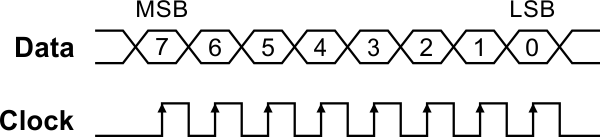
\includegraphics[width=0.6\textwidth]{images/FW/APA102.png}}\hfill
    \subfloat[\label{fig:APA102_1}] {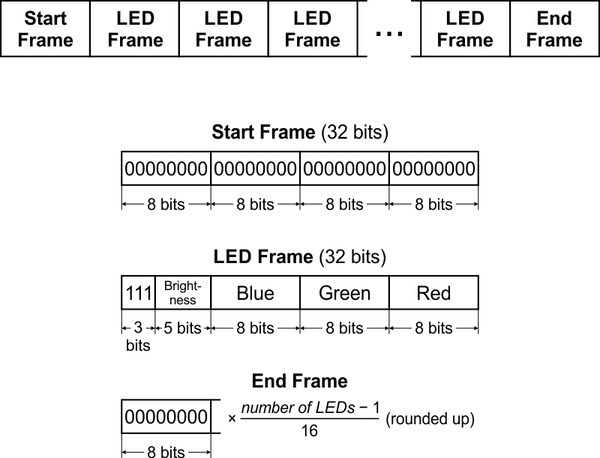
\includegraphics[width=0.7\textwidth]{images/FW/APA102_2.jpg}}\hfill
    \caption{APA102 communication protocol} 
    \label{fig:APA102}
\end{figure}   
   


    \subsubsection{Sound}
The Arduino Tone function and sound libraries have not been implemented yet for ESP32. In order to circumvent this problem, we use ESP32's LED PWN abilities to control our buzzer (described in Section \ref{subsubsec:hardware/esp32_capabilities}). With the PWM, the duty cycle and frequency can be set. We used a fixed duty cycle (which influences the loudness of sound) and used the frequency parameter to set up tones.


\lstinputlisting[style=Arduino, firstline=29, lastline=45]{code_snippets/arduino/Sound.ino}


\subsection{Next steps - functions to be implemented}
    \paragraph{Capacitive sensors calibration and touch/squeeze recognition} The capacitive touch sensors are the part currently requiring the most work. For China, we will test different parameter configurations in order to find the best sensitivity of the sensors within the final plush skin coming from industrial design. 
    \paragraph{WiFi save Smartconfig in EEPROM} As mentioned above, our goal for connectivity is to be able to remember a previously configured WiFi network by saving it in the microcontroller's EEPROM and retrieving it upon boot. This will allow users to configure the WiFi only once per location the toy will be used.
    \paragraph{Sleep functions} Currently, the toy is always either on or off and waiting for WiFi communication from server. Our goal for next semestre is to implement sleep modes so that a forgotten plush toy will not deplete its battery and the autonomy of the toy can be increased.
    \paragraph{Sound settings and implementing a proper loudspeaker} The current loudspeaker sounds "cheap" and the PWM signal makes it sound very electronic. As the plush toy is supposed to be a high-quality product, we should implement a better-sounding speaker and sounds. 
    \paragraph{Error checking} Currently, the game and message functions only check for basic errors. Some advanced error-checking should be implemented in order to avoid receiving and sending the wrong messages and having interactions not working properly.
    
    
    
